\documentclass[a4paper, 12pt]{article}
\usepackage[utf8]{inputenc}
\usepackage[T1]{fontenc}
\usepackage[scale=.8]{geometry}
\usepackage[french]{babel}
\usepackage{graphicx}

\title{Tunnel IPv6 sur IPv4}

\author{M1 Informatique \\\\ SCHNEEBERGER Thibault, CHAPUT Jean}
\date{}

\begin{document}
    \maketitle
    \newpage
    \tableofcontents
    \newpage

    \section{Configuration réseau}
    $$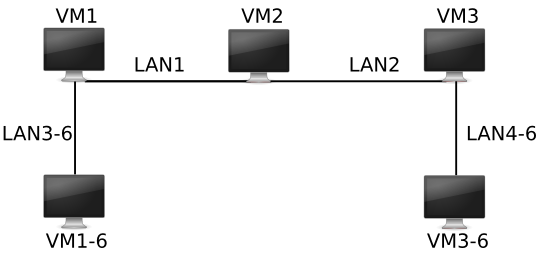
\includegraphics[scale=0.6]{images/topologie.png}$$
    \\
    Pour démarrer, on s'intéresse à la réalisation du réseau de 5 machines
    proposé dans l'énoncé du sujet dont le schéma se trouve juste au dessus. 
    Pour cela, on reprend notre configuration du TP précédent en y apportant 
    quelques modifications. Premièrement, on supprime la configuration de la 
    deuxième interface dans les fichiers de configuration ansible sur les 
    machines VM1.6 et VM3.6 car ces machines n'en auront plus la nécessité. 
    (Cela n'est pas nécessaire pour le bon fonctionnement mais ça permet de 
    faire un peu de propre). On supprime de plus les routes devenues obsolètes 
    permettant auparavant le passage par VM2.6 pour la communication en IPv6.

    \section{Interface TUN}
    Une fois notre configuration terminée avec ansible, on s'intéresse 
    maintenant à la création et à la configuration d'une interface virtuelle
    TUN qui nous permettra d'effectuer la communication entre l'espace noyau
    (d'où provient une trame échangée sur le réseau) vers l'espace utilisateur
    (où se trouvera le code de notre tunnel).

    \subsection{Création de l'interface}
    Afin de créer l'interface TUN, on récupère le code contenu dans le 
    fichier tunalloc.c. Celui-ci contient la fonction tun\_alloc et une 
    fonction principale main. Lorsque l'on regarde d'un peu plus près la 
    fonction tun\_alloc, on remarque que lors de son appel elle retourne
    un entier. Il s'agit du descripteur de fichier permettant la lecture
    ou bien l'écriture sur cette interface.

    \medbreak{}

    On crée donc une bibliothèque \textit{iftun}, c'est-à-dire un fichier
    d'en-tête iftun.h et un fichier source iftun.c afin d'y ajouter la fonction
    tun\_alloc. En plus de cela on crée un fichier principal avec une fonction 
    main nous permettant d'effectuer les tests de cette partie et les suivants.

    \subsection{Configuration de l'interface}
    Pour configurer l'interface TUN, on a besoin de lui attribuer une addresse
    IPv6. Nous utiliseront l'adresse \textit{fc00:1234:ffff::1} avec le masque
    en /64. Comme rappelé un peu plus haut il est aussi nécessaire de modifier
    les configurations créées au TP précédent car dans notre cas certaines 
    routes ne sont plus valides. Par exemple pour VM1 et VM1.6, dans le cas où
    ces machines voudraient communiquer avec VM3.6, elles ne pourront plus 
    passer par VM2.6.

    \medbreak{}

    On crée donc un script \textit{configure\_tun.sh} qui contiendra la commande
    \textit{ip address add fc00:1234:ffff::1/64 dev tun0}. Cela ne suffit pas 
    car lorsque l'interface TUN est créée, elle est désactivée. Pour l'activer 
    on rajoute une ligne de plus dans le script avec la commande \textit{ip 
    link set dev tun0 up}. La configuration est maintenant terminée.

    \medbreak{}

    Afin de tester notre configuration et après avoir lancé notre programme de 
    test sur VM1, on tente d'effectuer un \textit{ping6} de VM1.6 vers 
    l'interface tun0 sur VM1. Celui-ci se déroule dans problème et reçoit une 
    réponse. Cependant, si l'on effectue une capture wireshark sur VM1, on se 
    rend compte que les échanges ne passent pas par tun0. En effet, celle-ci ne
    capte aucune trame. Cela peut s'expliquer car lorsque la trame envoyée par 
    VM1.6 arrive sur VM1 par son interface eth2 (passerelle par défaut de 
    VM1.6) elle est désencapsulée afin de regarder qui est le destinataire pour
    pouvoir lui transmettre dans une nouvelle trame. Voyant que le destinataire
    est en réalité lui-même, le routeur VM1 peut traiter la demande et envoyer 
    sa réponse. Cela se déroule dans l'espace noyau.

    \medbreak{}

    On effectue ensuite le test en faisant \textit{ping6} depuis VM1 vers
    l'addresse \textit{fc00:1234:ffff::10}. Cette fois-ci le ping ne reçoit 
    pas de réponse mais en effectuant une analyse de paquets avec wireshark
    sur VM1, on se rend compte que les paquets sont transmis depuis 
    l'interface eth2 de VM1 vers tun0. Le ping ne reçoit ainsi pas de réponse 
    car pour le moment les paquets dans tun0 ne sont pas traités. Attention 
    car pour cette partie il faut bien penser à ajouter le drapeau de routage
    IPv6 sur VM1 (et par symétrie sur VM3) sinon la transmission entre 
    interfaces d'une même machine ne pourra pas s'effectuer. 

    \subsection{Récupération des paquets}
    Maintenant que l'on sait que les paquets sont redirigés sur l'interface
    virtuelle tun0 dont nous disposons du descripteur de fichier, on peut 
    s'intéresser à la récupération des informations dans tun0. On complète
    donc notre bibliothèque iftun avec une nouvelle fonction transfert qui
    permettra de transférer les données lues sur un descripteur de fichier
    source vers un descripteur de fichier destination.

    \medbreak{}

    On effectue donc le test de cette fonction avec comme descripteur de 
    fichier source celui retourné par la création de l'interface tun0 et
    comme descripteur de fichier destination 1 (qui correspond à la 
    sortie standard). On effectue à nouveau les pings réalisés précédemment
    depuis VM1.6. Au niveau du réseau rien ne change, Les captures sont 
    identiques. Cependant, on observe les paquets entrants sur tun0 s'afficher
    dans le terminal. Attention à bien filtrer l'affichage avec 
    \textit{hexdump} afin de rendre cela plus lisible.

    \medbreak{}

    Différentes options sont disponibles lorsque l'on crée l'interface 
    virtuelle. On peut utiliser les flags suivants: IFF\_TUN, IFF\_TAP et
    IFF\_NO\_PI. IFF\_TUN est celui que l'on utilise car il permet de 
    supprimer les en-têtes Ethernet afin de ne garder que le datagramme IP.
    IFF\_NO\_PI permet de retirer les 4 octets concernant la version du 
    protocole de couche IP. Le flag IFF\_NO\_PI peut s'ajouter en plus du 
    flag IFF\_TUN, les flags sont cumulables.

    \section{Un tunnel simple pour IPv6}

    Afin de faire communiquer VM1 et VM3 qui sont reliés par le biais de VM2
    en IPv4, on utilisera la connexion par socket à l'image d'un client et 
    d'un serveur. Pour cela on créera une nouvelle bibliothèque extremite avec
    un fichier d'en-têtes extremite.h et son fichier source extremite.c.

    \subsection{Redirection du traffic entrant}

    Afin de rediriger le traffic lu sur tun0 vers notre réseau IPv4, il nous
    faut créer une fonction extin qui aura en réalité un rôle de client et qui
    sera chargée d'ouvrir une connexion avec l'autre extrémité du tunnel afin
    de lui envoyer tout ce qui est lu. Après avoir ouvert une connexion 
    distante sur sa socket, on peut simplement effectuer un appel à notre 
    fonction transfert de la bibliothèque iftun. Celle-ci prend deux 
    descripteurs de fichiers en paramètres, le premier étant celui retourné par
    tun0 et le deuxième la socket en elle-même.

    \medbreak{}

    En plus de la fonction extin, il nous faut aussi une fonction extout qui 
    sera chargée du rôle de serveur et qui écoutera donc sur sa socket afin de 
    rediriger dans un premier temps vers la sortie standard (descripteur de 
    fichier 1) afin de vérifier que tout fonctionne correctement. La 
    redirection est ici aussi effectuée à l'aide de la fonction transfert de la
    bibliothèque iftun. À terme le transfert ne s'effectuera plus vers la sortie 
    standard mais bien sur le descripteur de fichier de tun0 afin de réinjecter
    notre datagramme IPv6 dans le réseau.

    \medbreak{}

    Lorque tout est  mis en place, c'est à dire que le programme de test est
    lancé en mode client sur VM1 et en mode serveur sur VM3, on peut effectuer 
    notre \textit{ping6} habituel depuis VM1.6 vers 
    \textit{fc00:1234:ffff::10}. Si l'on se place ensuite sur VM3, on voit 
    l'ensemble des paquets arriver depuis le tunnel s'afficher sur la sortie
    standard.

    \subsection{Redirection du traffic sortant}

    Maintenant qu'il est possible pour nous d'afficher le contenu du tunnel
    sur la sortie standard de VM3, on veut pouvoir le rediriger son interface
    virtuelle tun0. Cela aura pour but de réintégrer le datagramme IPv6
    transporté par le tunnel sur IPv4 dans le réseau IPv6. Pour cela il suffit
    de modifier la fonction extout de la bibliothèque extremite en effectuant
    un transfert non plus vers 1 (sortie standars) mais vers le descripteur de
    fichier retourné par tun0.

\end{document}